\documentclass[nooutcomes]{ximera}
%% handout
%% space
%% newpage
%% numbers
%% nooutcomes


\newcommand{\RR}{\mathbb R}
\renewcommand{\d}{\,d}
\newcommand{\dd}[2][]{\frac{d #1}{d #2}}
\renewcommand{\l}{\ell}
\newcommand{\ddx}{\frac{d}{dx}}
\newcommand{\dfn}{\textbf}
\newcommand{\eval}[1]{\bigg[ #1 \bigg]}

\usepackage{multicol}

\renewenvironment{freeResponse}{
\ifhandout\setbox0\vbox\bgroup\else
\begin{trivlist}\item[\hskip \labelsep\bfseries Solution:\hspace{2ex}]
\fi}
{\ifhandout\egroup\else
\end{trivlist}
\fi} %% we can turn off input when making a master document
\usepackage{fullpage}
\title{Section - 2.5:  Limits at Infinity}  

\begin{document}
\begin{abstract}		\end{abstract}
\maketitle

%problem1
\begin{problem}
	Select the meaning of $\lim_{x \to \infty} f(x)=6$.  Support your explanation graphically.

	\begin{enumerate}
	\item As $x$ becomes arbitrarily negatively large, $f(x)$ approaches $6$
	\item As $x$ becomes arbitrarily positively large, $f(x)$ approaches $6$
	\item As $x$ approaches 6, $f(x)$ becomes arbitrarily negatively large
	\item As $x$ approaches 6, $f(x)$ becomes arbitrarily positively large
	\end{enumerate}

	\begin{freeResponse}
	As $x$ becomes arbitrarily positively large, $f(x)$ approaches $6$.  Here are two examples of what this function might look like:
	\begin{image}
	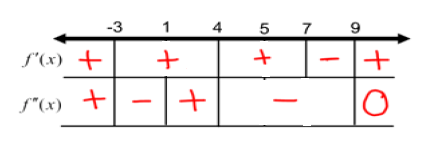
\includegraphics[scale=.5]{figure8.png}
	\end{image}
	\begin{image}
	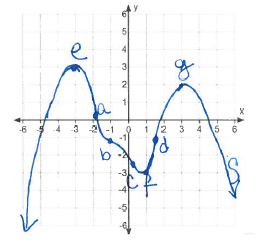
\includegraphics[scale=.5]{figure9}
	\end{image}
	\end{freeResponse}

\end{problem}

%problem2
\begin{problem}
Evaluate the following limits.
	\begin{enumerate}
		\item $\lim_{x \to \infty} \frac{\sqrt[3]{x^9+5}}{3x^3+ \sqrt{4x^6+1}}$
		\begin{freeResponse}
		\begin{align*}
		\lim_{x \to \infty} \frac{\sqrt[3]{x^9+5}}{3x^3+ \sqrt{4x^6+1}}
		&=\lim_{x \to \infty} \frac{\sqrt[3]{x^9+5}}{3x^3+ \sqrt{4x^6+1}}\cdot \frac{\frac{1}{x^3}}{\frac{1}{x^3}}\\
		&=\lim_{x \to \infty} \frac{\frac{\sqrt[3]{x^9+5}}{x^3}}{\frac{3x^3+ \sqrt{4x^6+1}}{x^3}}\\
		&=\lim_{x \to \infty}  \frac{\sqrt[3]{\frac{x^9+5}{x^9}}}{\frac{3x^3}{x^3}+ \sqrt{\frac{4x^6+1}{x^6}}}\\
		&=\lim_{x \to \infty}  \frac{\sqrt[3]{1+\frac{5}{x^9}}}{3+ \sqrt{4+\frac{1}{x^6}}}\\
		&=\frac{1}{3+ \sqrt{4}}\\
		&=\frac{1}{5}
		\end{align*}
		\end{freeResponse}

		\item $\lim_{x \to \infty} \frac{\sin{9x}}{5x}$
		\begin{freeResponse}
		 Since $-1 \le  \sin(9x) \le 1$ for all $x$ , and therefore $\frac{-1}{5x} \le  \sin(9x) \le \frac{1}{5x}$.\\
		  We have $\lim_{x \to \infty} \left(-\frac{1}{5x} \right) = 0$ and $\lim_{x \to \infty} \frac{1}{5x} = 0$.  The Squeeze theorem implies that
        \[
          \lim_{x \to \infty} \frac{\sin{9x}}{5x} = 0
        \]
		\end{freeResponse}
	\end{enumerate}
\end{problem}

%problem 3
\begin{problem}
The function $f$ defined by $\displaystyle f(x) = \frac{\sqrt{2x^2 + 1}}{3x-5}$.
  \begin{enumerate}
    \item
      Find all vertical asymptotes.  Justify using limits.
 \begin{freeResponse}
        Candidate for vertical asymptotes: $3x - 5 = 0 \implies x = 5/3$.

        Test of candidate $x = 5/3$:
        \begin{align*}
          &\lim_{x \to \frac{5}{3}^+} \frac{\sqrt{2x^2 + 1}}{3x-5} = \infty\\
	&\text{Because the limit is of the form:} \frac{\text{pos}}{0^+}\\
          &\implies \mbox{vertical asymptote at $x = 5/3$}
        \end{align*}

       \end{freeResponse}

    \item
      Find all horizontal asymptotes.  Justify using limits.
 

        \begin{freeResponse}
        Test of horizontal asymptote as $x \to \infty$:
        \begin{align*}
          \lim_{x \to \infty} \frac{\sqrt{2x^2 + 1}}{3x-5}
          &= \lim_{x \to \infty} \frac{\sqrt{2x^2 + 1}}{3x-5} \cdot \frac{\frac{1}{x}}{\frac{1}{x}} \\
          &= \lim_{x \to \infty}  \frac{\frac{\sqrt{2x^2 + 1}}{\sqrt{x^2}}}{3 - \frac{5}{x}}\\
          &= \lim_{x \to \infty}  \frac{\sqrt{2 + \frac{1}{x^2}}}{3 - \frac{5}{x}} \\
          &= \frac{\sqrt{2}}{3} \\
          &\implies \mbox{The line $y = \sqrt{2}/3$ is a horizontal asymptoteas $x \to \infty$.}
        \end{align*}

        Test of horizontal asymptote as $x \to -\infty$:
        \begin{align*}
          \lim_{x \to -\infty} \frac{\sqrt{2x^2 + 1}}{3x-5}
          &= \lim_{x \to -\infty} \frac{\sqrt{2x^2 + 1}}{3x-5} \cdot \frac{\frac{1}{x}}{\frac{1}{x}} \\
          &= \lim_{x \to -\infty}  \frac{\frac{\sqrt{2x^2 + 1}}{-\sqrt{x^2}}}{3 - \frac{5}{x}}\\
          &= \lim_{x \to -\infty}  \frac{-\sqrt{2 + \frac{1}{x^2}}}{3 - \frac{5}{x}} \\
          &= \frac{-\sqrt{2}}{3} \\
          &\implies \mbox{The line $y = -\sqrt{2}/3$ is a horizontal asymptote as $x \to -\infty$}
        \end{align*}
	
      \end{freeResponse}
 \end{enumerate}

    
\end{problem}

%problem4
\begin{problem}

  For the function $g$ defined by 
  \[
    g(t) = \frac{t^2 + 7t + 11}{t-3}
  \]
  \begin{enumerate}
    \item
      Find all vertical asymptotes.  Justify using limits.
      \begin{freeResponse}
        Candidates for vertical asymptote: $t - 3 = 0 \implies t = 3$.

        Test of candidate $t = 3$:
        \begin{align*}
          &\lim_{t \to 3^+} \frac{t^2 + 7t + 11}{t-3}= \infty \\
	&\text{Because the limit is of the form:} \frac{\text{pos}}{0^+}\\
          &\implies \mbox{vertical asymptote at $t = 3$}
        \end{align*}


      \end{freeResponse}


    \item

      Find all horizontal asymptotes and justify using limits.
      \begin{freeResponse}
	To find the limits, we need to divide the numerator and denominator by the highest power of $t$ in the denominator.
        \begin{align*} 
         &\lim_{t \to \infty} \frac{t^2 + 7t + 11}{t-3} = \lim_{t \to \infty} \frac{t + 7 + \frac{11}{t}}{1-\frac{3}{t}} = \infty \\
	&\text{Because the limit is of the form:} \frac{\infty}{\text{pos}}\\
          &\implies \mbox{no horizontal asymptotes as $t \to \infty$}
        \end{align*}

        \begin{align*}
         & \lim_{t \to -\infty} \frac{t^2 + 7t + 11}{t-3} = \lim_{t \to -\infty}\frac{t + 7 + \frac{11}{t}}{1-\frac{3}{t}} = -\infty \\
	&\text{Because the limit is of the form:} \frac{-\infty}{\text{pos}}\\
          &\implies \mbox{no horizontal asymptotes as $t \to -\infty$}
        \end{align*}
      \end{freeResponse}



  \end{enumerate}
\end{problem}


%problem5
\begin{problem}
 Sketch a possible graph of a function that satisfies all of the given properties.
  (You \emph{do not} need to find a formula for the function.)
  \begin{align*}
 	\lim_{x \to -2^-} f(x) &= \infty &   f(-2) &= -5 &  f(1) &= 2 \\
	 \lim_{x \to \infty} f(x) &= -\infty & \lim_{x \to -\infty} f(x) &= 4 & \lim_{x \to 5} f(x) &= \infty \\
	 \lim_{x \to 3} f(x) &= 3 & f(3) &=  1 &\\
	  \lim_{x \to -2^+}f(x)&=5  & f(4) &\text{ is undefined}& \lim_{x \to 4}f(x)&=3\\
  \end{align*}
  \begin{freeResponse}
      There are many correct solutions to this problem.
  One possible solution can be constructed as follows:
	First we draw the given points.  We'll also draw open brackets on the x-axis at $x=4$ since $f(x)$ is not defined at $x=4$ (This is seen in green.)
	\begin{image}
   	 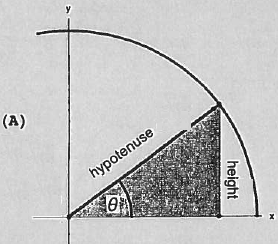
\includegraphics[scale = 0.4]{Figure10.png}   
	\end{image} 

	Then we draw the vertical  and horizontal asymptotes (in purple) and arrows indicating how the graph approaches the asymptote (in blue).  We also draw end-behavior as $x$ approaches $\infty$ and $-\infty$ (in blue).  We can also draw tails where we know limits at particular x-values.  Such as $ \lim_{x \to -2^+}f(x)=5$.
	\begin{image}
	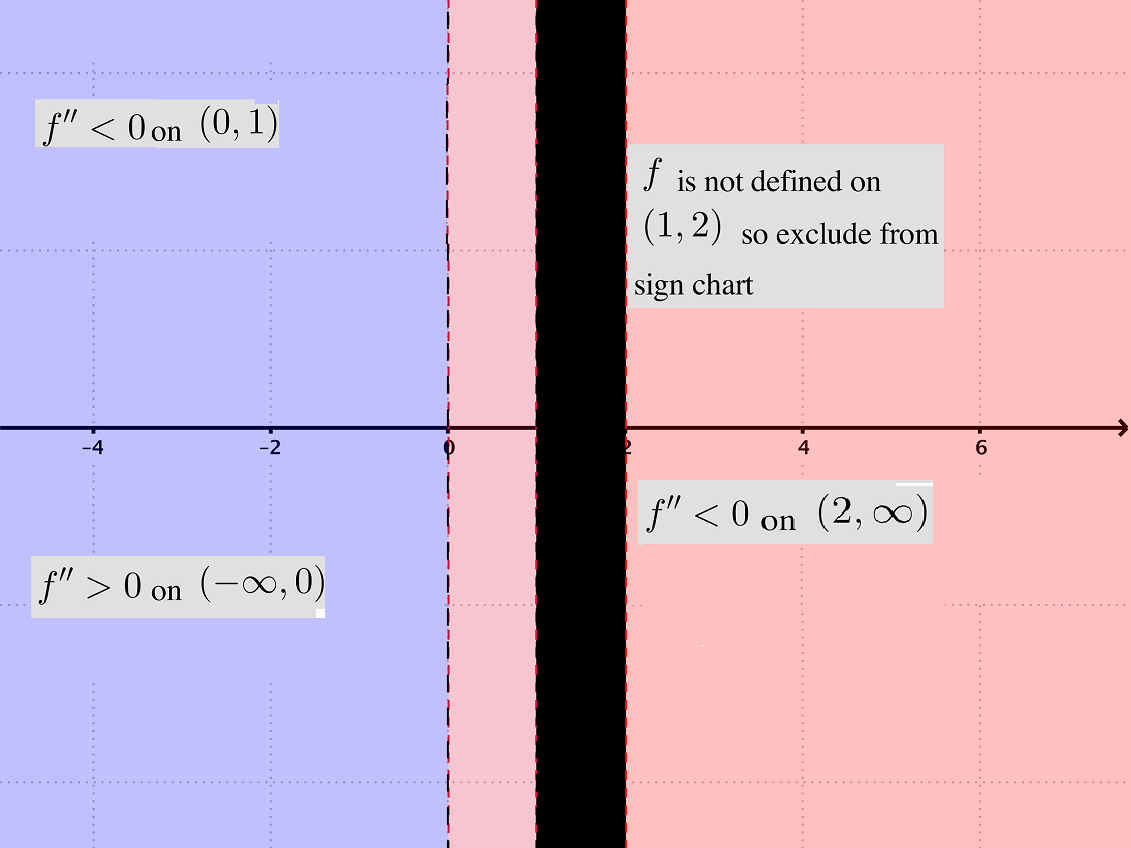
\includegraphics[scale = 0.4]{figure11.png}
	\end{image}

	Finally we connect our graph together (seen in blue)
	\begin{image}
    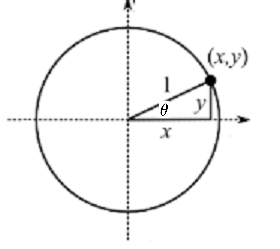
\includegraphics[scale = 0.4]{figure12.png}  
	\end{image}

  \end{freeResponse}
\end{problem}

























\end{document} 


















